% !TEX TS-program = pdflatex
% !TEX encoding = UTF-8 Unicode

% This is a simple template for a LaTeX document using the "article" class.
% See "book", "report", "letter" for other types of document.

\documentclass[10pt, a4paper]{article} % use larger type; default would be 10pt
\usepackage{fullpage}
\usepackage{graphicx}
\usepackage{subfigure}
\usepackage{algorithmic}
\usepackage{algorithm}
\usepackage{indentfirst}
\usepackage{graphicx} % support the \includegraphics command and options
%%% PACKAGES
\usepackage{booktabs} % for much better looking tables
\usepackage{array} % for better arrays (eg matrices) in maths
\usepackage{paralist} % very flexible & customisable lists (eg. enumerate/itemize, etc.)
\usepackage{verbatim} % adds environment for commenting out blocks of text & for better verbatim
% \usepackage{subfig} % make it possible to include more than one captioned figure/table in a single float
% These packages are all incorporated in the memoir class to one degree or another...
\usepackage{hyperref}
%%% HEADERS & FOOTERS
\usepackage{fancyhdr} % This should be set AFTER setting up the page geometry
\pagestyle{fancy} % options: empty , plain , fancy
\renewcommand{\headrulewidth}{0pt} % customise the layout...
\lhead{}\chead{}\rhead{}
\lfoot{}\cfoot{\thepage}\rfoot{}

%%% ToC (table of contents) APPEARANCE
\usepackage[nottoc,notlof,notlot]{tocbibind} % Put the bibliography in the ToC
\usepackage[titles,subfigure]{tocloft} % Alter the style of the Table of Contents
\renewcommand{\cftsecfont}{\rmfamily\mdseries\upshape}
\renewcommand{\cftsecpagefont}{\rmfamily\mdseries\upshape} % No bold!
%%% END Article customizations

%%% The "real" document content comes below...

\title{CIS 501 Final Project \\
Implementation and Analysis of the O-GEometric History Length branch predictor}
\author{Ben Charrow, Congyun Gu, Divya Kali Ranga, Xiaochuan Qin}
%\date{} % Activate to display a given date or no date (if empty),
         % otherwise the current date is printed

\begin{document}
\maketitle
\begin{abstract}

We studied and analyzed the Optimized GEometric History Length (O-GEHL) branch predictor described in Andre Seznec's paper \cite{seznec2005analysis} that efficiently exploits long global histories in the range of 100-200 bits.

The GEHL predictor features several predictor tables indexed through independent functions of the global branch history and branch address. The lengths of global history used form a geometric series (i.e., $L(i)=\alpha^{i-1}L(1)$) , allowing the GEHL predictor to efficiently capture correlation on recent as well as  old branch outcomes. The prediction is computed by passing the predictions on the predictor table through an adder.

The O-GEHL uses dynamic history fitting and dynamic threshold fitting to improve the ability of GEHL predictor in exploiting long histories.

Our experiments shows that GEHL and O-GEHL branch predictors significantly outperform baseline predictors, and their performance are influenced by several parameters. We also finds that the O-GEHL can be ahead pipelined using pipeline simulation model.
\end{abstract}

\section{Introduction}
Improvement in the accuracy directly translates to performance gain in modern predictors since all modern processors feature moderate issue width with deep pipelines. The O-GEHL predictor provides a prediction as a signed counter for each of its prediction tables. Hash functions are used to combine branch history, path history and instruction address. Heuristics methods are also used to dynamically adjust the prediction thresholds and the branch history length.

The implementation of O-GEHL predictor uses two metrics to evaluate its performance . The first one is the misprediction rate and the other is instruction per cycle(IPC). To evaluate the prediction accuracy of O-GEHL, we implement an infrastructure to compare O-GEHL to our existing predictors, namely, 2-bit saturating counter, gshare and tournament. This comparison gives us a baseline of the performance of O-GEHL.

We then explore the importance of four parameters that would impact O-GEHL predictor's performance. They are the number of tables $M$ used in prediction, width of the counter, history length, and threshold $\theta$ in updating the predictor tables. Section 4 describes our work in evaluating the performance of our GEHL/O-GEHL predictor using misprediction rate. We also discovered how O-GEHL predictor can be efficiently ahead pipelined using a pipeline simulation model using IPC.

\section{The GEHL Predictor}
\label{sec:gehl}
Compared with simple predictors we've built before, the O-GEHL predictor is quite complicated. In Seznec's implementation, several complex functions were added to extract information from index. To make sure that our implementations were correct, we worked in parallel, implementing two versions of GEHL separately and constantly compared the outputs to insure they were the same.   Using this approach, we detected and fixed several bugs, particularly in the index computation (Section ~\ref{sec:indexing}). Our final predictor catches most features described in Seznec's paper, and gives reliable performance in a series of experiments. This section briefly discusses the principle we used for implementation and focuses on the indexing function we've adapted from Seznec's work.

The GEHL predictor features $M$ distinct predictor tables $T_i$ , $0\leq i < M$.  Each of the tables has its own unique history length $L(i)$.  Together the lengths form a geometric series of the form $L(i)=\alpha^{i-1}L(1)$, $1\leq i < M$. $T_0$ uses a history length of 0.  To get an index for a branch, each tables uses its own index function -- which is dependent on $L(i)$ -- to combine information from the branch address, the branch history, and the path history.  The predictor tables store predictions in the form of signed counters. In order to compute a prediction , the counter value $C(i)$ is read on each table $T_i$ and the prediction is the sign of the sum $S$ of the $M$ counters $C(i)$, ($S = \frac{M}{2}+\sum_{0 \leq i < M} C(i)$). The prediction is taken if $S$ is 0 or positive and not-taken when S is negative.

The GEHL predictor updates itself on mispredictions or when the absolute value of the computed sum $S$ is smaller than a threshold $\theta$.  Algorithm\ref{alg:update} gives the exact update policy.
\begin{algorithm}[t]
  \label{alg:update}
  \caption{ GEHL update.  This algorithm updates the predictor if a branch is mispredicted or if the ``confidence'' of the prediction is below a certain threshold.}
  \begin{algorithmic}[1]
    \STATE Input: The current predicted direction of the branch $p$, the actual direction of the branch $a$, the sum of the tables for the predicted branch $S$, and the cutoff $\theta$.
    \STATE
    \IF{($p\neq a$) or ($|S| \leq \theta$)}
    \FOR{each $i$ in parallel}
      \IF{$a$ is taken}
        \STATE $C(i)=C(i)+1$
      \ELSE
        \STATE $C(i)=C(i)-1$
      \ENDIF
    \ENDFOR
    \ENDIF
  \end{algorithmic}
\end{algorithm}
\subsection{Indexing the Predictor}
\label{sec:indexing}
The main purpose of the GEHL predictor is to increase the overall performance of a branch predictor by exploiting drastically different history lengths.  This presents a problem when using the history as part of the index to the prediction tables.  Simpler schemes like gshare -- which use history lengths that are about equal to the number of index bits -- can simply XOR the branch history with other components in order to determine the index.  This will not work for GEHL, though, because typical configurations consider branch histories with more than 150 entries.  GEHL also uses the path history, which is the sequence of low order bits from both conditional and unconditional branches, to create the index.

\begin{algorithm}[t]
  \newcommand{\g}{\texttt{g}}
  \renewcommand{\c}{\texttt{c}}
  \caption{History compression.  $i$ is the table number.  $L(i)$ is the number of history bits that the table uses. $n$ is the number of index bits. \texttt{shift} and \texttt{lastDest} are parameters that must be less than $n$.  This algorithm effectively compresses the branch history for use as an index in the table.}
  \label{alg:compression}
  \begin{algorithmic}[1]
    \STATE Input: The current compressed history \c, and the global branch history \texttt{g} where \g[0] is the most recent branch direction.
    \STATE Output: A new compressed history
    \STATE
    \STATE $\c = (\c$ left-shifted by \texttt{shift} bits) XOR \g[0]
    \STATE $\c = \c\;$ XOR (\g[L(i)] left-shifted by \texttt{lastDest})
    \STATE $\c = \c\;$ XOR (\c right-shifted by $n$ bits)
    \STATE $\c = \c\;$ AND (bitmask of length $n$)
 \end{algorithmic}
\end{algorithm}

One simple approach to this problem would be to hash the full branch history down to the number of index bits.  However, as Seznec notes\cite{seznec2005analysis}\cite{ogehl} and we concur, such an approach would require a large number of additional logic gates and would significantly increase the latency of the instruction decode stage of the pipeline (or whatever pipeline stage branch prediction is performed in).  Such an approach is infeasible in practice.

O-GEHL addresses this problem by compressing the branch histories at each stage.\cite{cbp1}\cite{ogehl}\cite{seznec2005analysis} The exact compression algorithm is given in Algorithm\ref{alg:compression}, but the basic idea is relatively straight forward.  Each table stores its own version of the global branch history and incorporates new branches as they come in.  By shifting and masking bits depending on the history length used in the table, the history can be compressed so that its size equals the number of index bits for the table.  To actually compute the index for each table the predictor extracts bits from the path history, compressed branch history, and PC to create a bit string that is $3n$ bits long ($n$ being the number of bits used to index the table).  These bits are then compressed down to $n$ bits via a series of 3-way XOR gates and the result is used as an index into the table.  Like Seznec, we set the length of the used path history be $\min(16, L(i))$ for each table.

We used a slight modification of Seznec's approach in our implementation of the indexing function.  Our function simply XORs $n$ bits from the PC, $n$ bits from the compressed path history, and $n$ bits from the compressed branch history.  The primary difference is that this approach does not compose the various contributions first.  For example, if a table uses $n=8$ index bits and the table only uses $4$ bits of history, our implementation will mask off the 4 high order bits of the branch and path histories so that they are 0.  Seznec's approach is to take 8 additional bits from the PC, so that all $3n=24$ bits contain actual data.  As our results do not differ significantly from those reported by Seznec, we do not think the difference is particularly important.

\section{The O-GEHL predictor}
The O-GEHL predictor is an improved and more dynamic version of the GEHL predictor.  The update rule, possible table configurations, and index function are essentially the same.  The difference is that instead of using fixed values for the threshold cutoff $\theta$ and the length of the branch history, O-GEHL dynamically adjusts these parameters while a program is executing.  This adaptability enables a single O-GEHL predictor to perform close to the best performance of several different GEHL predictors across a wide variety of programs.

\subsection{Adapative threshold}
\label{sec:adaptT}
The value of $\theta$ controls whether or not the predictor is updated if a branch is correctly predicted (see \ref{alg:update}).  If its value is too low, the predictor will only update when a branch is mispredicted, which will result in the saturating counters hovering close to zero, making them more susceptible to noise. Conversely, if its value is too high the predictor will frequently update its table, causing the predictor to overfit to correctly predicted branches.  In our experimental evaluation, we found that the best value of $\theta$ changes from program to program (Table~\ref{table:bestTheta}).

To alleviate this issue, O-GEHL dynamically adjusts the value of $\theta$ in such a way that the number of updates on a miss-prediction are roughly equal to the number of updates on a correct prediction.  This approach is undoubtedly heurestic, but Seznec found it to be effective.\cite{seznec2005analysis}\cite{ogehl}  The basic idea is to maintain a saturating counter, the Threshold Counter (TC), whose value is increased or decreased depending on the cause of the update.  If TC becomes fully saturated one way or the other, then the value of theta is incremented or decremented appropriately.  The exact algorithm can be found in Algorithm~\ref{alg:dynT}.  Seznec suggested that using a 7-bit counter for TC was effective, and although we did not examine this parameter in detail, we obtained good experimental results using this value.

\begin{algorithm}[h]
  \caption{Dynamic $\theta$ adjustment.  This algorithm updates the value of $\theta$ so that the number of updates due to low confidence is roughly equal the number of updates due to mispredictions.}
  \begin{algorithmic}[1]
    \label{alg:dynT}
    \STATE Input: The actual direction of the branch $a$, the predictor's guess $p$, and the sum of all of the tables predictions $S$.
   \STATE
    \IF{$p\neq a$}
      \STATE $TC = TC + 1$
    \ELSIF{$|S|\leq\theta$}
      \STATE $TC = TC - 1$
    \ENDIF
    \IF{TC is saturated positive}
      \STATE $\theta=\theta+1$
      \STATE $TC=0$
    \ELSIF{TC is saturated negative}
      \STATE $\theta=\theta-1$
      \STATE $TC=0$
    \ENDIF
  \end{algorithmic}
\end{algorithm}


\subsection{Adaptive history}
\label{sec:adaptH}
O-GEHL is also able to dynamically adjust the history length that it uses in some of its tables.  The motivation for this ability is that some programs exhibit predictable behavior over the course of 300 branches, whereas some do not.  The only way for a predictor to be able to perform at its peak on both types of programs, while still exploiting history, is for it to dynamically adjust.  The O-GEHL accomplishes this by having some of its tables have two history lengths: a short one and a long one.  All of these tables will unanimously switch between their short length and long length depending on the value of a saturating counter. The long lengths are a continuation of the geometric series governed by $\alpha$ and $L1$, so the only additional parameters are the number of additional history lengths and the number of bits used in the saturating counter.

% how it is implemented
Clearly the crux of this approach is deciding when to switch.  As Seznec notes, programs that do not need longer history lengths will exhibit a high degree of aliasing (i.e. the same branches will consistently cause predictor updates).\cite{seznec2005analysis}\cite{ogehl} For programs requiring shorter histories, this effect will be most pronounced in the last table.  Similarly, if a wide variety of branches are causing predictor updates, it is an indication that a longer branch history will be beneficial.  O-GEHL measures this aliasing by recording the low-order bit of the PC whenever the predictor is updated, and storing this bit in an array indexed by the branch's index for the last table.  A saturating counter is used to track the source of mispredictions over time.  This counter is called the Aliasing Counter (AC).  Seznec reported that using 9 bits for the AC allowed the predictor to adapt when needed, but did not cause frequent length changes.  In our analysis, we do not examine either of these values.  The complete algorithm is given in Algorithim~\ref{alg:dynH}.

% how we did it for various table sizes
For our implementation of dynamic history fitting in the O-GEHL paper, we parameterized the number of additional history lengths used.  Seznec does not describe how these lengths should be spread for an arbitrary predictor, and so we chose to to evenly spread the additional history lengths over all of the tables aside from the first one and the last one.  The first is excluded because it never uses any history, while the last is excluded so that it can measure the aliasing.  As an example, if we had 6 tables and wanted 2 additional long history values, then table $T[2]$ would get a long history equal to $\alpha^{5}L(1)$ and table $T[4]$ would get a long history equal to $\alpha^{6}L(1)$.

\begin{algorithm}[h]
  \caption{Dynamic history adjustment.  Adjust whether or not the predictor uses the long version of table histories or the short one.}
  \label{alg:dynH}
  \begin{algorithmic}[1]

    \STATE Input: Whether or not the predictor was updated $u$, the \texttt{PC} of the branch, and the index $i$ of the branch in the last table.
    \STATE
    \IF{$u$ is true}
      \IF{Low order bit of $\texttt{PC}\neq\texttt{Tag}[i]$}
        \STATE $AC = AC - 4$
      \ELSE
        \STATE $AC = AC + 1$
      \ENDIF
      \IF{AC is saturated positive}
        \STATE Set tables to use long history
      \ELSIF{AC is saturated negative}
        \STATE Set tables to use short history
      \ENDIF
    \ENDIF
  \end{algorithmic}
\end{algorithm}

\section{Evaluation}
\label{sec:eval}
We evaluated both GEHL and O-GEHL in a variety of ways across all of the traces provided by the course staff.  For GEHL we examined how the history length (as determined by $\alpha$ and $L1$), the value of $\theta$, the number of bits used for the saturating counters and the number of tables affect the prediction accuracy.  For O-GEHL, we examined the impact of dynamically adjusting the history length as well as dynamically adjusting the value of $\theta$.  In addition to predictor accuracy, we also see how various predictors affect the IPC using a simulation of a super-scalar out of order processor.  When appropriate, we compared GEHL and O-GEHL against a variety of baseline predictors.

Due to time constraints, we did not run our simulations on all of the microops in all of our benchmarks.  Instead, we created a short and long version for each trace and for each experiment, chose one or the other.  Details about the traces we used, as well as their lengths, are in Table\ref{table:traces}.  In each of our figures, average accuracies are reported as the unweighted mean across all traces that were used.
\begin{table}
  \centering
  \begin{tabular}{l|r|r|r}
    Trace Name & Total Operations & Long Version & Short Version \\ \hline
    gcc & 50M & 50M & 10M \\
    go & 100M & 100M  & 10M \\
    hmmer & 100M & 100M & 10M \\
    libquantum & 100M & 50M & 10M\\
    sjeng & 100M &50M & 10M \\
    sphinx3 &100M & 50M & 10M \\
    art & 100M & 50M & 10M\\
    mcf & 100M & 100M & 10M\\
 \end{tabular}
 \caption{Traces used throughout the experiments.  Depending on the experiment, either a version with a larger number of microops was used or one with a shorter number of operations was used.}
 \label{table:traces}
\end{table}

Overall our results agree with those reported by Seznec.\cite{seznec2005analysis}\cite{ogehl}

\subsection{Prediction accuracy against baseline predictors}
In order to compare the prediction accuracies of various predictors, we ran
each of them across the traces by varying the cache sizes. Long version of
traces are used in this experiments, of which each trace is at the size of 50M
or 100M. For GEHL and O-GEHL, we use the best parameters getting from our
experiments, namely, the number of table used is around 6, the $\alpha$ is set
to 2, and the saturating counter width is set to 4.From the results, we could
infer that as the cache size increases, the GEHLand the O-GEHL predictors
outperform all of the other predictors. For instance, O-GEHL's performance is
the best of all predictors we've compared when the predictor size is bigger
than 4K-bit. Although we did not perform the experiments on very long traces,
we expect the O-GEHL predictor to eventually outperform all predictors since
its begins exploiting very long global histories.  See
Figure~\ref{fig:comparison} for full results.
\begin{figure}[h]

  \subfigure[Branch predictor accuracy (long traces)]
  {\label{subfig:graph1-acc}\scalebox{0.8}{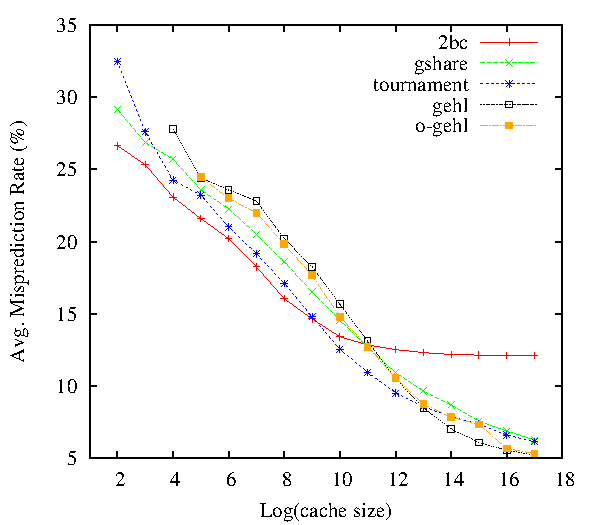
\includegraphics{figs/graph1-acc.pdf}}}
  \subfigure[Standard deviation of predictor accuracy.]
  {\label{subfig:graph1-stddev}\scalebox{0.8}{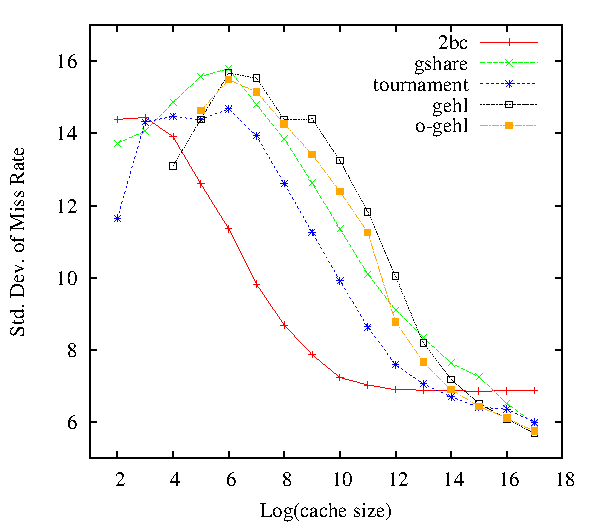
\includegraphics{figs/graph1-stddev.pdf}}}

  \subfigure[Branch predictor accuracy (long traces)  Zoomed in.]
  {\label{subfig:graph1-acc-zoom}\scalebox{0.8}{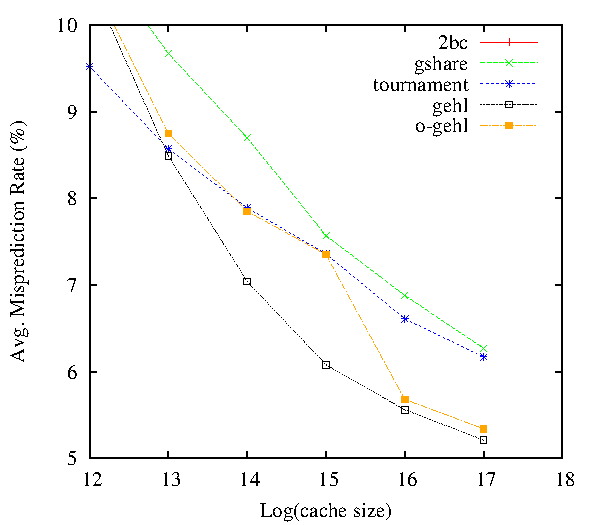
\includegraphics{figs/graph1-acc-zoom.pdf}}}
  \subfigure[Standard deviation of predictor accuracy. Zoomed in.]
  {\label{subfig:graph1-stddev-zoom}\scalebox{0.8}{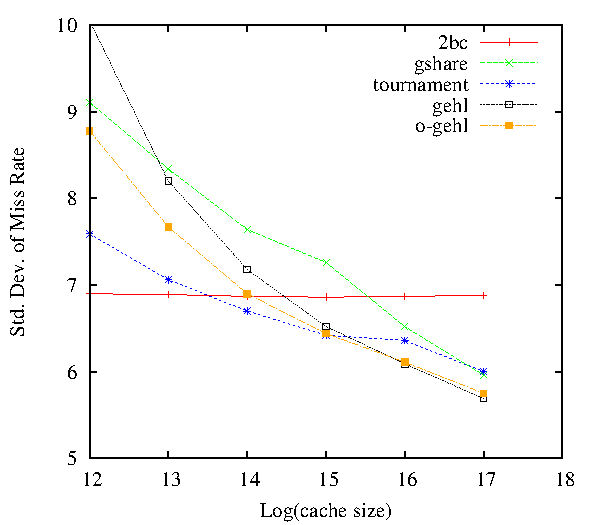
\includegraphics{figs/graph1-stddev-zoom.pdf}}}

  \caption{Branch predictor compassion.  Each data point in \ref{subfig:graph1-stddev} reports the standard deviation of the accuracy of the same predictor in \ref{subfig:graph1-acc}.  \ref{subfig:graph1-acc-zoom} and \ref{subfig:graph1-stddev-zoom} show a closeup of the large predictors' performance.  Overall GEHL outperforms O-GEHL until large predictor sizes are reached, at which point O-GEHL does about as well.  However, they both outperform the other branch predictors.}
  \label{fig:comparison}
\end{figure}

\subsection{Update threshold}
As discussed in Section~\ref{sec:gehl}, GEHL updates when a misprediction occurs or when the magnitude of the sum from all of the tables is below a threshold $\theta$.  Figure~\ref{fig:theta} shows several GEHL predictors across various sizes and with various values of $\theta$.  In the range that we explored, $\theta$ doesn't have a significant impact on the average accuracy.  However, a more detailed analysis of our results show that the best value of $\theta$ varies from trace to trace, just as Seznec indicated. Table 2 shows the best $\theta$ value in our experiments for a 1-Kbit GEHL predictor.
\begin{table}
  \centering
  \begin{tabular}{l|r}
    Trace Name(Short Version) & Best $\theta$ \\ \hline
    gcc & 8 \\
    go &  10 \\
    hmmer &10 \\
    libquantum & 4\\
    sjeng  & 4\\
    sphinx3  &4 \\
    art  &10\\
    mcf  & 10\\
 \end{tabular}
 \caption{$\theta$ with best performance for a 1-Kbit GEHL predictor of each trace.}
 \label{table:bestTheta}
\end{table}
\begin{figure}[h]
  \subfigure[Branch predictor accuracy (short traces)]
  {\scalebox{0.8}{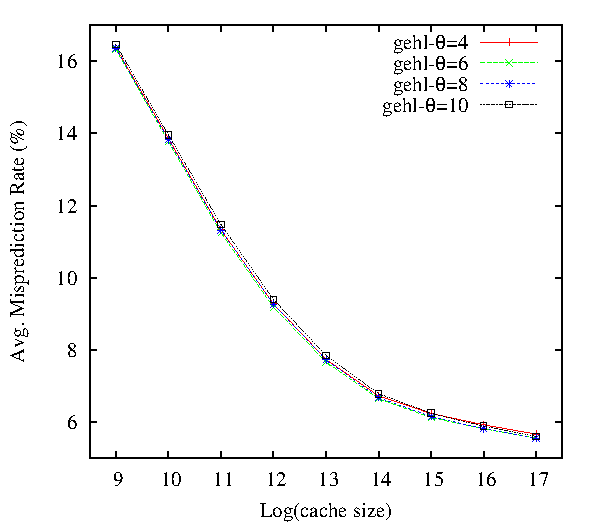
\includegraphics{figs/graph2-acc.pdf}}}
  \subfigure[Standard deviation of branch predictor accuracy]
  {\scalebox{0.8}{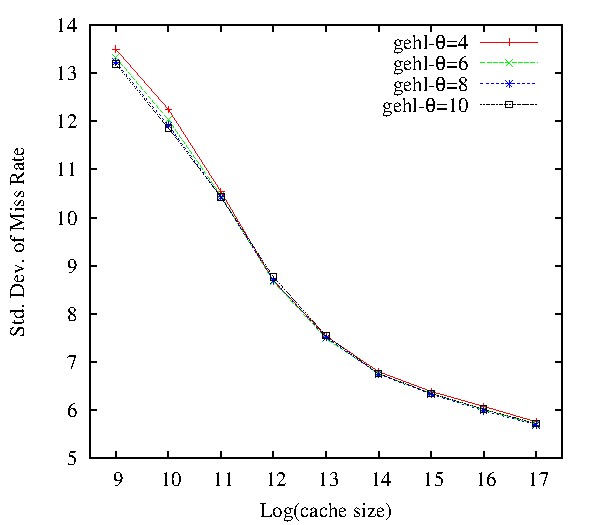
\includegraphics{figs/graph2-stddev.pdf}}}

  \caption{How the value of $\theta$ affects GEHL's prediction accuracy.  Overall, $\theta$ does not have a substantial affect on the accuracy of the branch predictors.}
  \label{fig:theta}
\end{figure}


\subsection{Size of Saturating Counters}
Determining the best size of the saturating counters for a GEHL predictors is a tradeoff between space complexity and performance. Figure~\ref{fig:sb} shows our experimental results for saturating counters with various widths. Performance improves significantly when the the counter increases from from 3-bits to 4-bits.  The standard deviation also drops significantly, indicating that the predictor performs much better across all traces.  However, the performance gain of using 5 bits or more is limited, whereas the added size is substantial as each entry of each table uses a counter.  This data suggests that using 4-bit counters is a good tradeoff.  Seznec reported similar results.

\begin{figure}[h]
  \subfigure[Branch predictor accuracy (short traces)]
  {\scalebox{0.8}{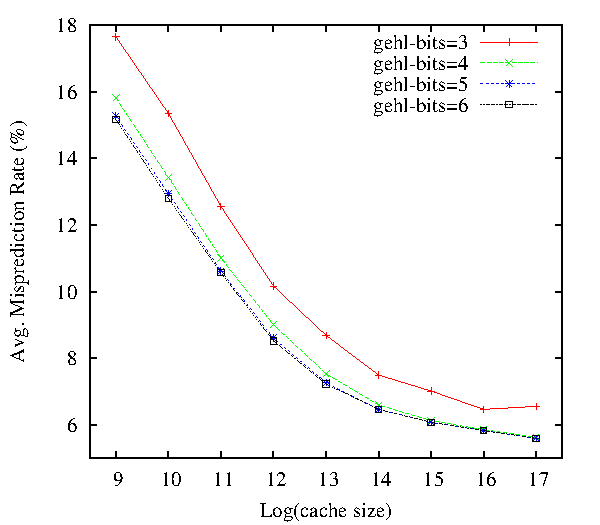
\includegraphics{figs/graph3-acc.pdf}}}
  \subfigure[Standard deviation of branch predictor accuracy]
  {\scalebox{0.8}{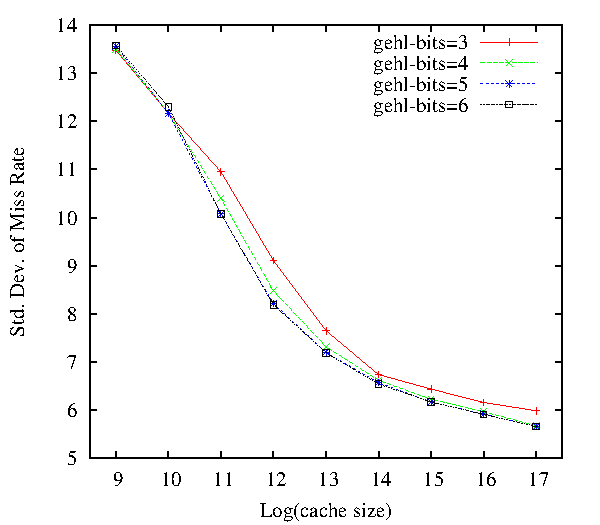
\includegraphics{figs/graph3-stddev.pdf}}}

  \caption{How the size of each table's saturating counters affect GEHL's prediction accuracy.}
  \label{fig:sb}
\end{figure}


\subsection{History length}
The length of each history table used in GEHL is determined by a geometric series based on $\alpha$. From Figure~\ref{fig:alpha}, we see that $\alpha=2.0$ gives the best results for all sizes of the cache.  Smaller values of $\alpha$, such as 1.2 work well when the storage budget is around 1K bits, and large $\alpha$, such as $\alpha$ = 3.0 gives competitive accuracy when the cache size is larger than 16 Kbits. This finding corresponds with Seznec's work as well.  It is worth mentioning that these experiments were done using 6 tables.  If this number had been larger, using a smaller $\alpha$ may have been advantageous because it would capture a finer range of history lengths.
\begin{figure}[h]
\subfigure[Branch predictor accuracy (short traces)] {\scalebox{0.8}{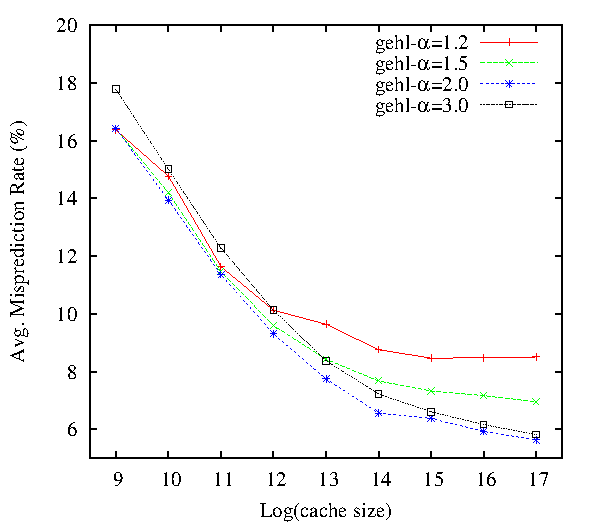
\includegraphics{figs/graph4-acc.pdf}}}
\subfigure[Standard deviation of branch predictor accuracy]
{\scalebox{0.8}{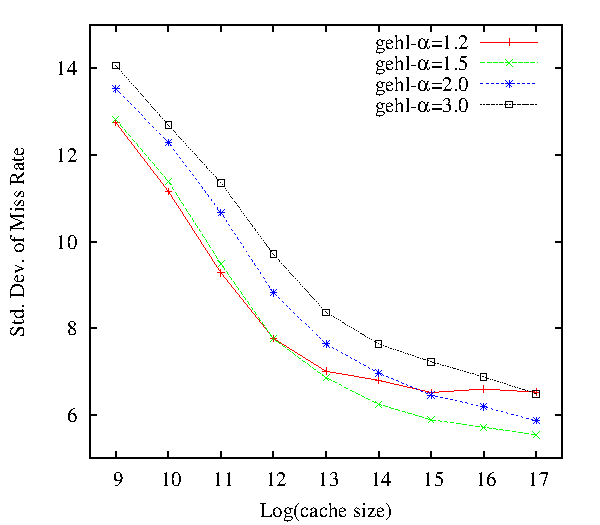
\includegraphics{figs/graph4-stddev.pdf}}}

\caption{How $\alpha$, the growth rate of the history length, affects GEHL's prediction accuracy.}
\label{fig:alpha}
\end{figure}

\subsection{Number of Tables}
The number of tables has the single greatest impact on the performance and space complexity of the predictors.  Figure~\ref{fig:tables} contains data for a wide range of table sizes.  The number of index bits used in the predictor was adjusted to insure relevant comparisons between predictors.  For the set of considered benchmark traces, we found 6 tables to perform the best when the predictor storage budget was small (less than or equal to 96 Kbits).  For such a storage budget, doubling the number of predictor tables, but halving each individual table indexing bits does not improved any performance.  When the storage budget is very small (less than 16Kbits), a 4 table configuration outperforms than 6 table configuration.  Not surprisingly, the general trend is that for large storage budgets, using more tables results in higher accuracy.

\begin{figure}[h]
  \subfigure[Branch predictor accuracy (short traces)]
  {\scalebox{0.8}{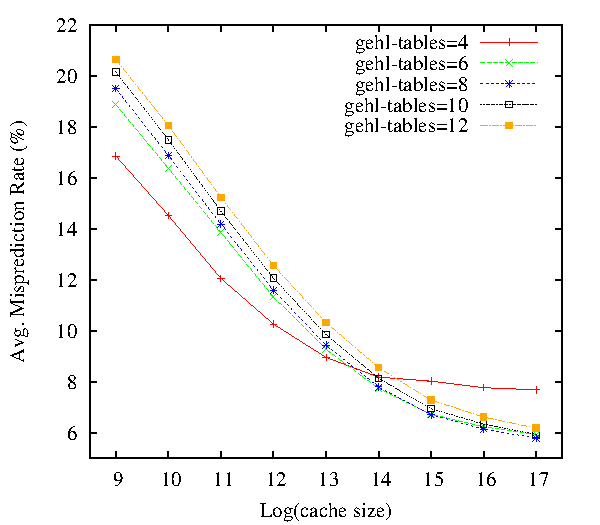
\includegraphics{figs/graph5-acc.pdf}}}
  \subfigure[Standard deviation of branch predictor accuracy]
  {\scalebox{0.8}{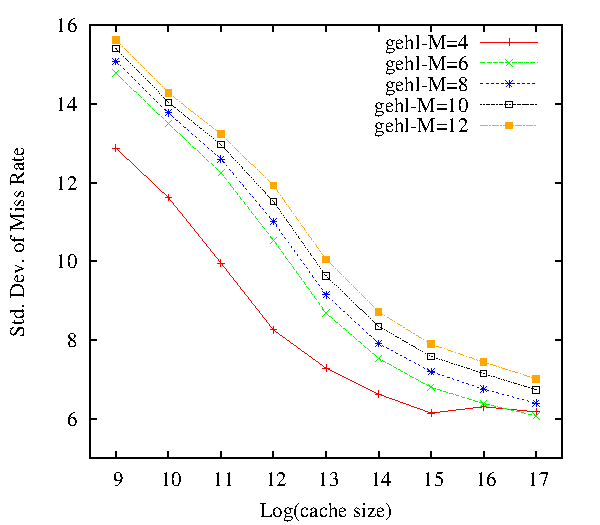
\includegraphics{figs/graph5-stddev.pdf}}}
  \caption{How the number of tables affects GEHL's prediction accuracy.}
  \label{fig:tables}
\end{figure}

\subsection{Adaptive Update Threshold and Adaptive History Length}
Two important changes were introduced in optimizing the original GEHL to O-GEHL.  One is the dynamic threshold fitting policy and the other is adaptive history length.  As we described in Section~\ref{sec:adaptT}, the best value of $\theta$ varies from trace to trace. Figure~\ref{fig:adaptT} shows a comparison between two GEHL predictors with different values of $\theta$ as well as an O-GEHL predictor which dynamically updates the threshold.  In general, O-GEHL performs about as well as the best fixed $\theta$ for each trace. In order to insure that the differences in performance were only due to adjustments of $\theta$, we disabled the dynamic history component of O-GEHL to collect this data.

Figure~\ref{fig:adaptH} shows a comparison between an O-GEHL predictor which adapts its history length as described in Section~\ref{sec:adaptH} and two separate GEHL predictors with vastly different history lengths.  In our experiment, though dynamically fitting history length reduces space complexity, its performance is not better than our best fixed history length growth rate $\alpha=2.0$. This is mainly because history information is lost during our indexing information extraction process, which we discussed in Section~\ref{sec:indexing}.

\begin{figure}[h]
  \centering
  \scalebox{0.8}{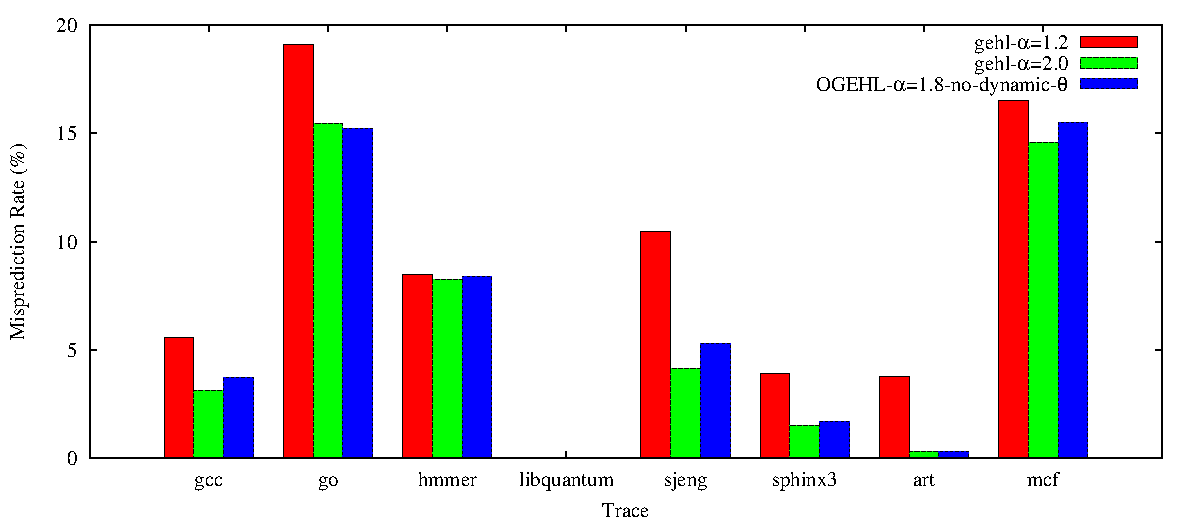
\includegraphics{figs/graph6.pdf}}

  \caption{Performance of O-GEHL with adaptive history length.  Adaptive $\theta$ is not used.  Adaptive history length is not used. All other parameters are the same and each of the predictors is 64Kbits.  This data was collected on the short traces.}
 \label{fig:adaptH}
\end{figure}

\begin{figure}[h]
  \centering
  \scalebox{0.8}{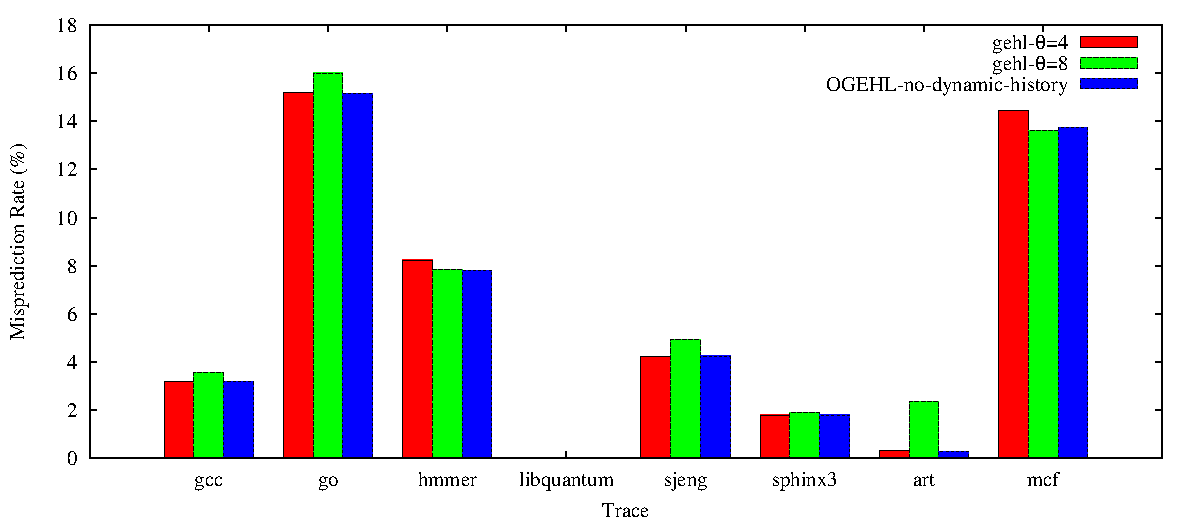
\includegraphics{figs/graph7.pdf}}

  \caption{Performance of OGEHL with adaptive $\theta$.  Adaptive history length is not used. All other parameters are the same and each of the predictors is 64Kbits.  This data was collected on the short traces.}
 \label{fig:adaptT}
\end{figure}

\subsection{Performance Impacts}
While branch prediction accuracies are important, in some sense the real
measure of a predictor is how much it increases the IPC of a processor.
Consequently, we evaluated the GEHL and O-GEHL predictors with the best
parameters that we found against a gshare predictor using a simple super scalar
out of processor simulation.  The results are summarized in
Figure~\ref{fig:ipc}.  Overall, both O-GEHL and GEHL give similar IPC results
across a variety of reorder buffer sizes.  Both of them outperform the gshare
predictor.  Because all of the predictors are the same size, and have a similar
standard deviation across the various traces that were used, we conclude that
either predictor would be a better choice for a modern processor.

One interesting fact which is somewhat obscured by the average in
Figure~\ref{subfig:ipc2} is how well the branch predictors perform on some of
the traces.  In both the sphinx3 and art traces, GEHL and O-GEHL achieve an IPC
of that is within 5\% of the idealized case.  Gshare also does well, but is
still outperformed by the geometric predictors.
\begin{figure}[h]
  \subfigure[Average uIPC]{\label{subfig:ipc2}\scalebox{0.8}{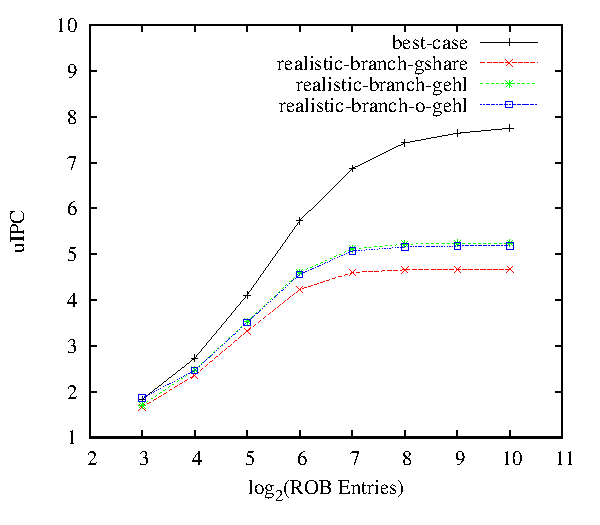
\includegraphics{figs/graph8.pdf}}}
  \subfigure[Standard Deviation of uIPC]{\scalebox{0.8}{\includegraphics{figs/graph8-stddev.pdf}}}

  \caption{Impact of branch predictors on IPC.  On a simulation of a super scalar out of order processor with realistic branch prediction and memory, both GEHL and O-GEHL improve IPC compared to a reference gshare predictor, regardless of the number of entries in the reorder buffer.  `best-case' is a processor with perfect branch prediction and memory scheduling.  All predictors are 64Kbits big and the data was obtained using the long version of the art, gcc, go and sphinx3 traces.}
 \label{fig:ipc}
\end{figure}

\section{Related work}
Our work mainly depends on Andre Seznec's design and implementation of the O-GEHL predictor, which he submitted to the the first Championship Branch Prediction competition.\cite{seznec2005analysis}\cite{cbp1}\cite{ogehl} In \cite{seznec2005analysis}, he credits research done over a 15 year period for his design.  Among these are the use of combining the results from multiple predictors, which was first introduced in McFarling's seminal work.\cite{mcfarling1993combining}

\section {Conclusion}
In this report, we described our implementations of GEHL and O-GEHL branch predictor, and evaluated the performance compared with baseline branch predictors. Significant performance improvement acheived by GEHL and O-GEHL over 8 distinct long traces. Also, by exploring four important parameters used in GEHL and O-GEHL predictor, we found the best value of threshold $\theta$ varies from trace to trace, and the best value of history length growth rate $\alpha$ is 2.0. The most cost-effective number of tables is 6-bit and the best size of saturating counters is 4-bit. These findings are consistent with Seznec's results. Adaptive history length and adaptive threshold also improved performance during our experiments, but not as signifcant as suggested by previous researches. We also ensured that GEHL and  OGEHL can be pipelined ahead to increase the IPC. Overall, GEHL and OGEHL performs better than baseline predictors in our experiments, yet more complicated features, such as the indexing algorithm should be considered carefully in real implementation.

\bibliographystyle{abbrv} % format names like so: S. Teller
\bibliography{biblio}

\end{document}
